\state{Bhabha scattering (Peskin \& Schroeder 5.2)}{
	Compute the differential cross section $\dv*{\sig}{(\cos\tht)}$ for Bhabha scattering, $\elp \elm \to \elp \elm$.  You may work in the limit $\Ecm \gg \me$, in which it is permissible to ignore the electron mass.  There are two Feynman diagrams; these must be added in the invariant matrix element before squaring.  Be sure that you have the correct relative sign between these diagrams.  The intermediate steps are complicated, but the final result is quite simple.  In particular, you may find it useful to introduce the Mandelstam variables $s$, $t$, and $u$.  Note that, if we ignore the electron mass, $s + t + u = 0$.  You should be able to cast the differential cross section into the form
	\eq{
		\dv{\sig}{(\cos\tht)} = \frac{\pi \alp^2}{s} \brac{ u^2 \paren{ \frac{1}{s} + \frac{1}{t} }^2 + \paren{ \frac{t}{s} }^2 + \paren{ \frac{s}{t} }^2 }.
	}
	Rewrite this formula in terms of $\cos\tht$ and graph it.  What feature of the diagrams causes the differential cross section to diverge as $\tht \to 0$?
}

\sol{
	The two Feynman diagrams are the $s$- and $t$-channel diagrams~\cite[p.~157]{Peskin}
	\eq{
		\centergraphics{diag/ee_s_chan}
		\qquad \text{and} \qquad
		\centergraphics{diag/ee_t_chan}.
	}  
	The interaction Hamiltonian for QED is Peskin \& Schroeder~(4.129),
	\eq{
		\Hint = \int \ddcx e \psib \gamm \psi \Asm,
	}
	so the interaction is $\psib \Asm \gamm \psi$~\cite[p.~226]{Schwartz}.  Now we can write the matrix element for the interaction:
	\eq{
		\mel*{\vp, \vkk}{(\psib \Asm \gamm \psi)_x (\psib \Asm \gamm \psi)_y}{\vp', \vkk'}.
	}
	By Peskin \& Schroeder~(4.118),
	\al{
		\ket*{\vp, \vkk} &\sim \apdag \akdag \ket{0}, &
		\bra*{\vp', \vkk'} &\sim \bra{0} \akp \app.
	}
	Then the contractions for the $s$-channel diagram are
	\eq{
		\ev*{\wick{\c2{\akp} \c1{\app} (\c1{\psib} \Asm \gamm \c2{\psi})_x} \wick{(\c2{\psib} \Asm \gamm \c1{\psi})_y \c1{\apdag} \c2{\akdag}}}{0}.
	}
	For the $t$ channel,
	\al{
		\ev*{\wick{\c2{\akp} \c1{\app} (\c4{\psib} \Asm \gamm \c2{\psi})_x (\c1{\psib} \Asm \gamm \c3{\psi})_y \c3{\apdag} \c4{\akdag}}}{0}
		&= -\ev*{\wick{\c2{\akp} \c1{\app} (\Asm \gamm \c2{\psi} \c4{\psib})_x (\c1{\psib} \Asm \gamm \c3{\psi})_y \c3{\apdag} \c4{\akdag}}}{0} \\
		&= \ev*{\wick{\c2{\akp} \c1{\app} (\Asm \gamm \c2{\psi})_x \c1{\psib}_y} \wick{\c2{\psib}_x (\Asm \gamm \c1{\psi})_y \c1{\apdag} \c2{\akdag}}}{0} \\
		&= - \ev*{\wick{\c2{\akp} \c1{\app} \c1{\psib}_y (\Asm \gamm \c2{\psi}} \wick{\c2{\psib})_x (\Asm \gamm \c1{\psi})_y \c1{\apdag} \c2{\akdag}}}{0}.
	}
	We needed to swap the order of adjacent fields three times, which gives an overall minus sign~\cite[p.~118]{Peskin}.  This means we subtract the $t$ channel diagram:
	\eq{
		\centergraphics{diag/ee_s_chan} \quad - \quad \centergraphics{diag/ee_t_chan}.
	}
	The matrix element for the $s$ channel is the same as Peskin \& Schroeder~(5.1),
	\eq{
		\frac{i e^2}{s} \vbk \gamm \up \ubpp \gamsm \vkp.
	}
	For the $t$ channel, it is~\cite[p.~153]{Peskin}
	\eq{
		\frac{i e^2}{t} \ubpp \gamm \up \vbk \gamsm \vkp
	}
	where we have used the Mandelstam variables~\hl[cite].  Their difference is
	\eq{
		i \cM = i e^2 \brac{ \frac{\vbk \gamm \up \ubpp \gamsm \vkp}{s} - \frac{\ubpp \gamm \up \vbk \gamsm \vkp}{t} },
	}
	which means~\cite[p.~132]{Peskin}
	\eq{
		-i \cMs = -i e^2 \brac{ \frac{\ubp \gamm \vk \vbkp \gamsm \upp}{s} - \frac{\ubp \gamm \upp \vbkp \gamsm \vk}{t} }.
	}
	Then
	\al{
		\abs{\cM}^2 &= e^4 \left[ \frac{\vbk \gamm \up \ubpp \gamsm \vkp \ubp \gamn \vk \vbkp \gamsn \upp}{s^2} - \frac{\vbk \gamm \up \ubpp \gamsm \vkp \ubp \gamn \upp \vbkp \gamsn \vk}{s t} \right. \\
		&\hspace{1.5em} \left. \phantom{=\ } - \frac{\ubpp \gamm \up \vbk \gamsm \vkp \ubp \gamn \vk \vbkp \gamsn \upp}{s t} + \frac{\ubpp \gamm \up \vbk \gamsm \vkp \ubp \gamn \upp \vbkp \gamsn \vk}{t^2} \right].
	}
	Note that~\cite[p.~132, 153]{Peskin}
	\al{
		\sumspins \vbk \gamm \up \ubpp \gamsm \vkp \ubp \gamn \vk \vbkp \gamsn \upp &= \Tr( \ksl \gamm \psl \gamn ) \Tr( \psl' \gamsm \ksl' \gamsn ), \\
		\sumspins \ubpp \gamm \up \vbk \gamsm \vkp \ubp \gamn \upp \vbkp \gamsn \vk &= \Tr( \psl' \gamm \psl \gamn ) \Tr( \ksl \gamsm \ksl' \gamsn ),
	}
	where we have taken $m \to 0$.  Writing the other two using components,
	\al{
		\sumspins \brac{ \vbk \gamm \up \ubpp \gamsm \vkp \ubp \gamn \upp \vbkp \gamsn \vk + \cc }
		&= \sumssp \sumrrp \brac{ \vbsar \gammsab \usbs \ubscspp \gamsmcd \vsdrp \ubses \gamnef \usfsp \vsgrp \gamsngh \vshr + \cc } \\
		&= \sumssp \sumrrp \brac{ \vshr \vbsar \gammsab \usbs \ubses \gamnef \usfsp \ubscspp \gamsmcd \vsdrp \vsgrp \gamsngh + \cc} \\
		&= \ksl_{h a} \gammsab \psl_{b e} \gamnef \psl'_{f c} \gamsmcd \ksl'_{d g} \gamsngh + \cc \\
		&= \Tr( \ksl \gamm \psl \gamn \psl' \gamsm \ksl' \gamsn ) + \cc
	}
	where we have used Peskin \& Schroeder~(5.3),
	\al{
		\sums \usp \ubsp &= \psl + m, &
		\sums \vsp \vbsp &= \psl - m,
	}
	and $m = 0$.  This gives us the matrix element
	\eq{
		\abs{\cM}^2 = e^4 \paren{ \frac{\Tr( \ksl \gamm \psl \gamn ) \Tr( \psl' \gamsm \ksl' \gamsn )}{s^2} - \frac{\Tr( \ksl \gamm \psl \gamn \psl' \gamsm \ksl' \gamsn ) + \cc}{s t} + \frac{\Tr( \psl' \gamm \psl \gamn ) \Tr( \ksl \gamsm \ksl' \gamsn )}{t^2} }.
	}
	We need to average over spins: $\sumspins \abs{\cM}^2 / 4$~\cite[p.~132]{Peskin}.  From (5.70) and (5.71),
	\al{
		\frac{1}{4} \sumspins \frac{e^4}{s^2} \Tr( \ksl \gamm \psl \gamn ) \Tr( \psl' \gamsm \ksl' \gamsn ) &= \frac{8 e^4}{s^2} \brac{ \paren{ \frac{t}{2} }^2 + \paren{ \frac{u}{2} }^2 }, \\
		\frac{1}{4} \sumspins \frac{e^4}{t^2} \Tr( \psl' \gamm \psl \gamn ) \Tr( \ksl \gamsm \ksl' \gamsn ) &= \frac{8 e^4}{t^2} \brac{ \paren{ \frac{s}{2} }^2 + \paren{ \frac{u}{2} }^2 }.
	}
	For the remaining terms, we adapt Peskin \& Schroeder~(5.69),
	\al{
		s &= (p + k)^2
		= (p' + k')^2, &
		t &= (p' - p)^2
		= (k' - k)^2, &
		u &= (k' - p)^2
		= (p' - k)^2.
	}
	For the $s$ channel in the massless limit~\cite[p.~156]{Peskin},
	\al{
		t &= -2 p \cdot p'
		= -2 k \cdot k', &
		u&= -2 p \cdot k'
		= -2 k \cdot p'.
	}
	Note that
	\al{
		\Tr( \ksl \gamm \psl \gamn \psl' \gamsm \ksl' \gamsn ) &= \ksa \psb \psr' \kss' \Tr( \gama \gamm \gamb \gamn \gamr \gamsm \gams \gamsn ) \\
		&= -2 \ksa \psb \psr' \kss' \Tr( \gama \gamr \gamn \gamb \gams \gamsn ) \\
		&= -8 \ksa \psb \psr' \kss' \Tr( \gama \gamr \gbs ) \\
		&= -8 \ksa \psb \psr' \kpb \Tr( \gama \gamr ) \\
		&= -32 \ksa \psb \psr' \kpb \gar \\
		&= -32 \ksa \ppa \psb \kpb \\
		&= -32 (k \cdot p') (p \cdot k') \\
		&= -8 u^2,
	}
	where we have used Peskin \& Schroeder~(5.9),
	\al{
		\gamm \gamn \gamr \gamsm &= 4 \gnr, &
		\gamm \gamn \gamr \gams \gamsm &= -2 \gams \gamr \gamn,
	}
	and (5.5), $\Tr(\gamm \gamn) = 4 \gmn$.  Then the matrix element is
	\aln{
		\frac{1}{4} \sumspins \abs{\cM^2} &= \frac{8 e^4}{s^2} \brac{ \paren{ \frac{t}{2} }^2 + \paren{ \frac{u}{2} }^2 } + \frac{4 e^4}{s t} u^2 + \frac{8 e^4}{t^2} \brac{ \paren{ \frac{s}{2} }^2 + \paren{ \frac{u}{2} }^2 } \notag \\
		&= 2 e^4 \brac{ \paren{ \frac{t}{s} }^2 + \frac{u^2}{s^2} + 2 \frac{u^2}{s t} + \paren{ \frac{s}{t} }^2 + \frac{u^2}{t^2} } \notag \\
		&= 2 e^4 \brac{ u^2 \paren{ \frac{1}{s^2} + 2 \frac{1}{s t} + \frac{1}{t^2} } + \paren{ \frac{t}{s} }^2 + \paren{ \frac{s}{t} }^2 } \notag \\
		&= 32 \pi^2 \alp^2 \brac{ u^2 \paren{ \frac{1}{s} + \frac{1}{t} }^2 + \paren{ \frac{t}{s} }^2 + \paren{ \frac{s}{t} }^2 }. \label{ans2a}
	}
	By Peskin \& Schroeder~(4.85), the differential cross section for four particles of the same mass is
	\eq{
		\dv{\sig}{\Omg} = \frac{\abs{\cM}^2}{64 \pi^2 \Ecm^2}.
	}
	In the center-of-mass frame, $\Ecm = (p + k) = \sqrt{s}$.  Feeding in Eq.~\refeq{ans2a},
	\eq{
		\dv{\sig}{\Omg} = \frac{1}{64 \pi^2 \Ecm^2} \frac{1}{4} \sumspins \abs{\cM^2}
		= \frac{\alp^2}{2 s} \brac{ u^2 \paren{ \frac{1}{s} + \frac{1}{t} }^2 + \paren{ \frac{t}{s} }^2 + \paren{ \frac{s}{t} }^2 }.
	}
	Noting that $\ddOmg = \ddcost \ddphi$ and $\int \ddphi = 2\pi$, we integrate over $\phi$ to find
	\eqn{ans2b}{
		\ans{ \dv{\sig}{(\cos\tht)} = \frac{\pi \alp^2}{s} \brac{ u^2 \paren{ \frac{1}{s} + \frac{1}{t} }^2 + \paren{ \frac{t}{s} }^2 + \paren{ \frac{s}{t} }^2 } }
	}
	as desired. \qed
	
	From Peskin \& Schroeder~(5.72),
	\al{
		s &= \Ecm^2, &
		t &= -2 \abs{\vp}^2 (1 - \cos\tht), &
		u &= -2 \abs{\vp}^2 (1 + \cos\tht).
	}
	Feeding these into Eq.~\refeq{ans2b},
	\aln{
		\dv{\sig}{(\cos\tht)} &= \frac{\pi \alp^2}{\Ecm^2} \brac{ 4 \abs{\vp}^4 (1 + \cos\tht)^2 \paren{ \frac{1}{\Ecm^2} - \frac{1}{2 \abs{\vp}^2 (1 - \cos\tht)} }^2 + \paren{ -\frac{2 \abs{\vp}^2 (1 - \cos\tht)}{\Ecm^2} }^2 + \paren{ -\frac{\Ecm^2}{2 \abs{\vp}^2 (1 - \cos\tht)} }^2 } \notag \\
		&= \ans{ \frac{4 \pi \alp^2 \abs{\vp}^4}{\Ecm^2} \brac{ \paren{ \frac{(1 + \cos\tht)^4}{\Ecm^2} - \frac{(1 + \cos\tht)^4}{2 \abs{\vp}^2 (1 - \cos\tht)} }^2 + \paren{ \frac{1 - \cos\tht}{\Ecm^2} }^2 + \paren{ \frac{\Ecm^2}{1 - \cos\tht} }^2 }. } \label{ans2}
	}
	A graph is shown in Fig.~\ref{f2}.  The differential cross section diverges as $\tht \to 0$ since the photon in the diagrams is nearly on shell; that is, $q^2 \to 0$~\cite[p.~155]{Peskin}.  When the mediating photon is massless~(on shell), electrons that are separated by an infinite distance can still scatter off each other.  Since they are so far apart, however, the angle of scattering approaches 0.  Since any electron anywhere in the universe may be scattering off another given electron with $\tht \approx 0$, the scattering cross section must blow up there.
	
	\begin{figure} \centering
		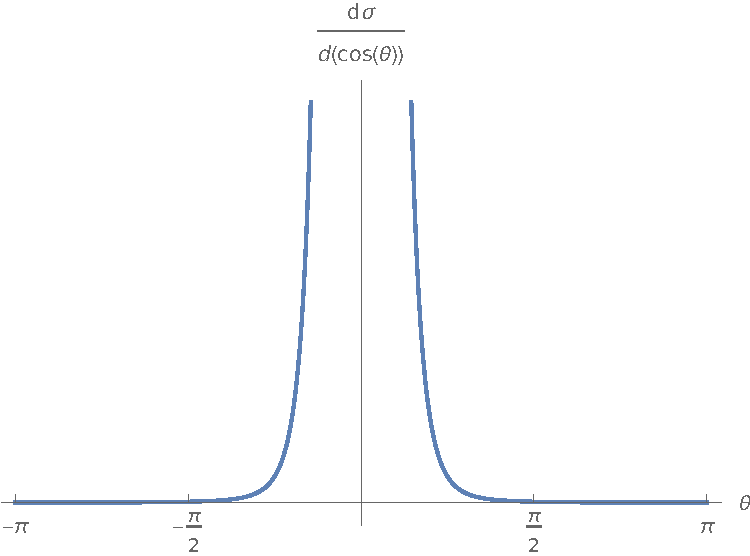
\includegraphics[width=0.4\textwidth]{2}
		\caption{Graph of Eq.~\refeq{ans2} showing divergence as $\tht \to 0$.}
		\label{f2}
	\end{figure}
	
	\bigskip\bigskip\bigskip
}